\documentclass{article}
\usepackage[utf8]{inputenc}
\usepackage{graphicx,subcaption}

%\usepackage{indentfirst} for APA margins and French indention
\usepackage{url}
%-------------------------------------------------------------------------------
% Configuring customized document margins
%-------------------------------------------------------------------------------
\usepackage{geometry}
\addtolength{\oddsidemargin}{-.75in}
\addtolength{\evensidemargin}{-.75in}
\addtolength{\textwidth}{1.4in}

\addtolength{\topmargin}{-0.25in}
\addtolength{\textheight}{1.65in}

%-------------------------------------------------------------------------------
% Configuring colors to make Python codes easy readable
%-------------------------------------------------------------------------------
\usepackage{listings}
\usepackage{color}

%-------------------------------------------------------------------------------
% Title region
%-------------------------------------------------------------------------------
\title{
UANL - FIME\\ 
Optimization on networks flows\\
Networks representation using graph theory \\
}
\author{Aned Esquerra Arguelles}
\date{\today}

\begin{document}
\raggedright
\maketitle

\section*{Introduction}
With its basic foundations in discrete mathematics, geometry and topology among others,  graph theory  has its very beginnings in 1736; the first documented application: the solution of the original problem of  the seven Koenigsberg  bridges, published by Leonhard Euler.\linebreak

Nowadays, this field of knowledge has evolved in one of the most interesting, important and challenging branch of mathematics and computational sciences, widely used in almost every aspects of real life.\linebreak 

Due to its tremendous impact and application, graphs, the nucleus of this established theory, are everywhere. Networks as part of optimization science.\linebreak

This working paper meant to be brief review of some general categories of graphs thru real-life examples coded and visualized with the help Python programming language, using \textbf{networkx} \cite{networkx} and  \textbf{matplotlib}\cite{matplotlib} references, samples, tutorials and packages for this purpose. \cite{autor2014}

\section{Acyclic undirected graphs}

Acyclic undirected simple graphs are widely used in design applications: when it is important to show to some executive stuff a brief model of the situation to solve, in other cases are just a tool to understand some processes, the relations between categories or concepts.\linebreak

Generally the direction of vertices between nodes it is not as important as the existence of themselves, most of the times exist a bidirectional relationship between the concepts, ideas or objects associated to the nodes.\linebreak  

Conceptual and mind maps, organization charts, computer network topology schemes, electrical circuits, phones lines, representation of chemical compounds, maps for subways stations and their connections, etc., are just few examples of the applications of this. \linebreak

A graphical representation of the example related to the family of graph reviewed in this section is a brief scheme of the former structural computers network topology proposed to the University Corporation of Meta, which can be observed in figure ~\ref{fig:AUSG}  on page ~\pageref{fig:AUSG}.\linebreak

\lstinputlisting[language=Python, caption=Python code associated to the graphical representation of UNIMETA computers network topology.]{codes/NF_H01_sect01.py}

\begin{figure}[!ht]
  \includegraphics[width=.8\columnwidth]{images/NF_H1_graph_sect01.eps}
  \caption{Pseudo-representation of UNIMETA network topology using acyclic undirected simple graph.}
  \label{fig:AUSG}
\end{figure}

\section{Cyclic undirected graphs}

\section{Reflexive undirected graphs}

\section{Acyclic directed graphs}

A graphical representation of the example related to the family of graph reviewed in this section is a brief scheme of the former structural computers network topology proposed to the University Corporation of Meta, which can be observed in figure ~\ref{fig:AUSG}  on page ~\pageref{fig:AUSG}.\linebreak

\lstinputlisting[language=Python, caption=Python code associated to the graphical representation of mathematical expression (tmp+x)*(pos - t^2).]{codes/NF_H01_sect04.py}

\begin{figure}[!ht]
  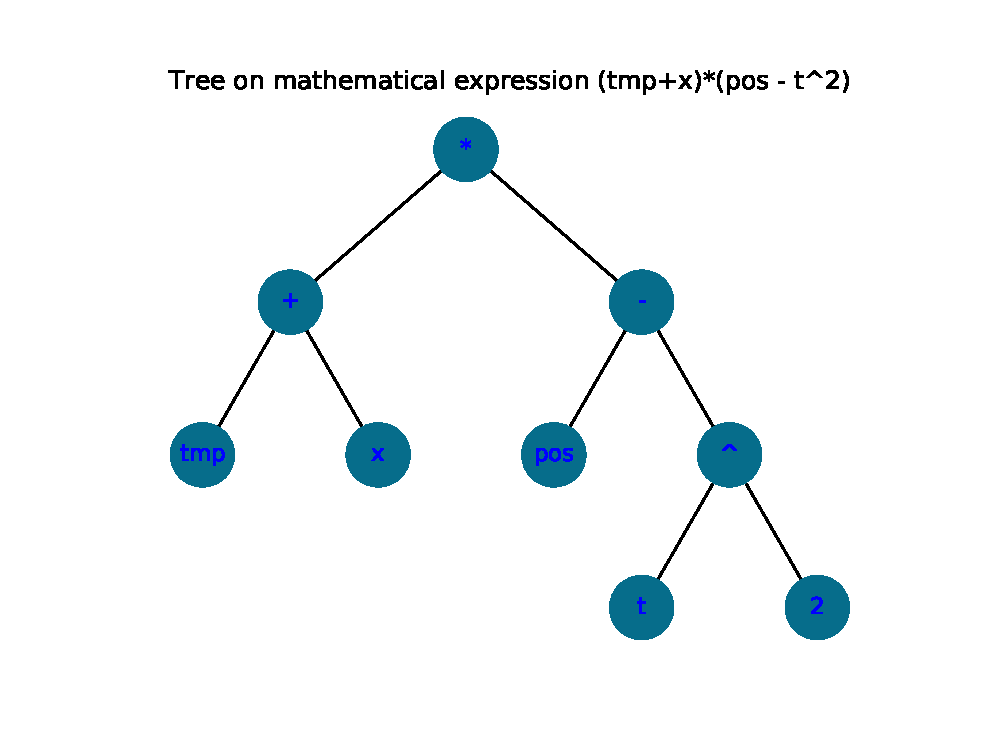
\includegraphics[width=.8\columnwidth]{images/NF_H1_graph_sect04.eps}
  \caption{Representation of the tree resulting in the analysis of mathematical expression (tmp+x)*(pos - t^2) using acyclic directed graph.}
  \label{fig:CDSG01}
\end{figure}

\section{}
\section{}
\section{}
\section{}
\section{}
\section{}
\section{}
\section{}


%-------------------------------------------------------------------------------
% References
%-------------------------------------------------------------------------------
\newpage
\bibliography{NF_HWI}
\bibliographystyle{plain}



\end{document}